\documentclass[border=6pt]{standalone}
\usepackage{fontspec}
\setmainfont{Times New Roman}
\usepackage{graphicx}
\usepackage{tikz}
\usetikzlibrary{arrows.meta,calc,fit,positioning,shapes.geometric}
\usepackage{pgfplots}
\pgfplotsset{compat=1.18}
\usepackage{amsmath,amssymb}
\usepackage{array}
\usepackage{booktabs}
\usepackage{xcolor}
\graphicspath{{figures/}{figures/ch3/}{figures/ch4/}{figures/apx/}}
\newcommand{\degreeC}{\ensuremath{^\circ\mathrm{C}}}
\newcommand{\figsource}[1]{}
\tikzset{
  thesis box/.style={
    draw,
    rounded corners=1pt,
    align=center,
    inner sep=4pt,
    minimum height=0.36in,
    font=\small
  },
  thesis process/.style={
    thesis box,
    fill=gray!8
  },
  thesis decision/.style={
    diamond,
    draw,
    aspect=2,
    align=center,
    inner sep=2pt,
    font=\small,
    fill=gray!8
  },
  thesis arrow/.style={
    -{Latex[length=2.2mm]},
    line width=0.65pt
  },
  thesis bus/.style={
    line width=0.8pt
  }
}
\newcommand{\socketCharPlot}[2]{%
  \begin{tikzpicture}
    \begin{axis}[
      width=0.95\textwidth,
      height=2.65in,
      xmin=0,
      xmax=#2,
      ymin=26,
      ymax=58,
      xlabel={Time (min)},
      ylabel={Temperature (\degreeC)},
      grid=both,
      major grid style={line width=0.2pt,draw=gray!45},
      minor grid style={line width=0.1pt,draw=gray!20},
      tick label style={font=\scriptsize},
      label style={font=\small},
      legend style={
        font=\scriptsize,
        draw=none,
        at={(0.5,1.03)},
        anchor=south,
        legend columns=3,
        /tikz/every even column/.append style={column sep=0.35em}
      },
      legend cell align={left}
    ]
      \addplot[black,thick] table[x=time,y=ntc] {figures/ch4/data/char_#1_normal.dat};
      \addlegendentry{Normal NTC}
      \addplot[black,thick,dashed] table[x=time,y=terminal] {figures/ch4/data/char_#1_normal.dat};
      \addlegendentry{Normal terminal}
      \addplot[gray!70!black,thick] table[x=time,y=ntc] {figures/ch4/data/char_#1_corroded.dat};
      \addlegendentry{Corroded NTC}
      \addplot[gray!70!black,thick,dashed] table[x=time,y=terminal] {figures/ch4/data/char_#1_corroded.dat};
      \addlegendentry{Corroded terminal}
      \addplot[black,densely dotted,thick] coordinates {(0,38.2) (#2,38.2)};
      \addlegendentry{38.2\degreeC}
    \end{axis}
  \end{tikzpicture}%
}

\newcommand{\socketProtectionPlot}[2]{%
  \begin{tikzpicture}
    \begin{axis}[
      width=0.95\textwidth,
      height=2.85in,
      xmin=0,
      xmax=#2,
      ymin=26,
      ymax=58,
      xlabel={Time (min)},
      ylabel={Temperature (\degreeC)},
      grid=both,
      major grid style={line width=0.2pt,draw=gray!45},
      minor grid style={line width=0.1pt,draw=gray!20},
      tick label style={font=\scriptsize},
      label style={font=\small},
      legend style={
        font=\scriptsize,
        draw=none,
        at={(0.5,1.03)},
        anchor=south,
        legend columns=3,
        /tikz/every even column/.append style={column sep=0.35em}
      },
      legend cell align={left}
    ]
      \addplot[black,thin,densely dotted] table[x=time,y=ntc] {figures/ch4/data/protect_#1_normal.dat};
      \addlegendentry{Normal NTC}
      \addplot[black,thick] table[x=time,y=estimated] {figures/ch4/data/protect_#1_normal.dat};
      \addlegendentry{Normal estimate}
      \addplot[black,thick,dashed] table[x=time,y=terminal] {figures/ch4/data/protect_#1_normal.dat};
      \addlegendentry{Normal terminal}
      \addplot[gray!70!black,thin,densely dotted] table[x=time,y=ntc] {figures/ch4/data/protect_#1_corroded.dat};
      \addlegendentry{Corroded NTC}
      \addplot[gray!70!black,thick] table[x=time,y=estimated] {figures/ch4/data/protect_#1_corroded.dat};
      \addlegendentry{Corroded estimate}
      \addplot[gray!70!black,thick,dashed] table[x=time,y=terminal] {figures/ch4/data/protect_#1_corroded.dat};
      \addlegendentry{Corroded terminal}
      \addplot[black,densely dashdotted,thick] coordinates {(0,40) (#2,40)};
      \addlegendentry{40\degreeC trip}
    \end{axis}
  \end{tikzpicture}%
}

\begin{document}

  \centering
  \begin{minipage}{0.47\textwidth}
    \centering
    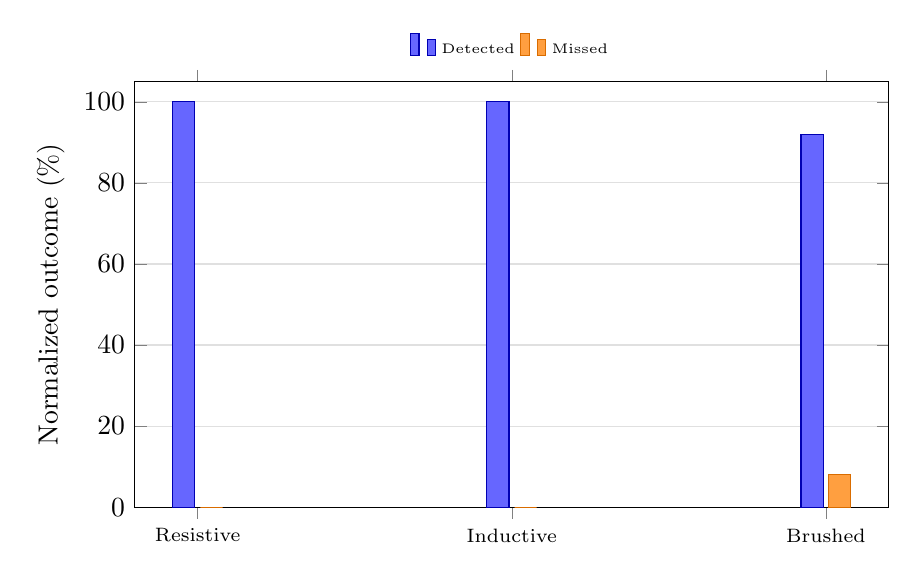
\begin{tikzpicture}
      \begin{axis}[
        ybar,
        width=0.92\linewidth,
        height=2.75in,
        ymin=0,
        ymax=105,
        ylabel={Normalized outcome (\%)},
        symbolic x coords={Resistive,Inductive,Brushed},
        xtick=data,
        x tick label style={font=\scriptsize},
        ymajorgrids=true,
        grid style={black!12},
        bar width=8pt,
        legend style={font=\tiny,at={(0.5,1.03)},anchor=south,legend columns=2,draw=none},
      ]
        \addplot[fill=blue!60,draw=blue!70!black] coordinates {(Resistive,100) (Inductive,100) (Brushed,92)};
        \addplot[fill=orange!75,draw=orange!85!black] coordinates {(Resistive,0) (Inductive,0) (Brushed,8)};
        \legend{Detected,Missed}
      \end{axis}
    \end{tikzpicture}
    {\small (a) Arc Trials}
  \end{minipage}\hfill
  \begin{minipage}{0.47\textwidth}
    \centering
    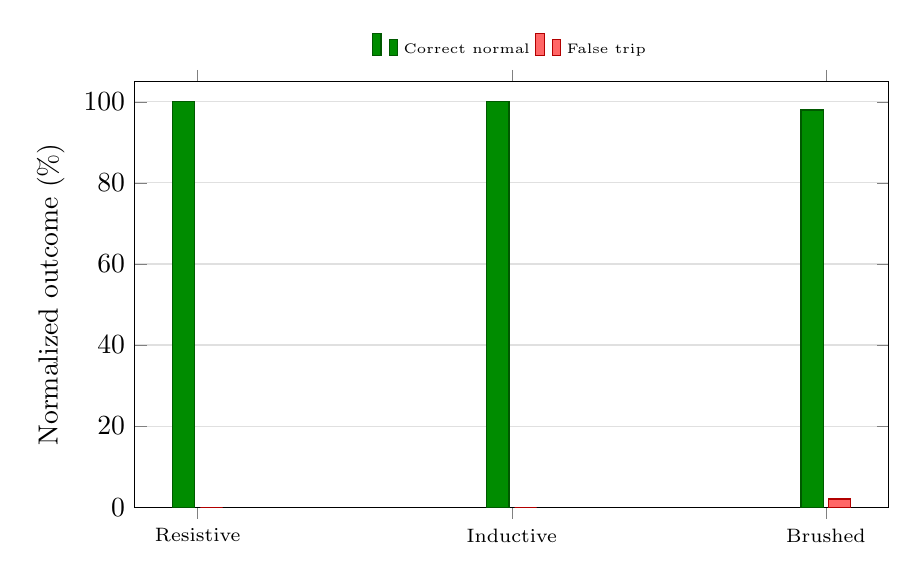
\begin{tikzpicture}
      \begin{axis}[
        ybar,
        width=0.92\linewidth,
        height=2.75in,
        ymin=0,
        ymax=105,
        ylabel={Normalized outcome (\%)},
        symbolic x coords={Resistive,Inductive,Brushed},
        xtick=data,
        x tick label style={font=\scriptsize},
        ymajorgrids=true,
        grid style={black!12},
        bar width=8pt,
        legend style={font=\tiny,at={(0.5,1.03)},anchor=south,legend columns=2,draw=none},
      ]
        \addplot[fill=green!55!black,draw=green!35!black] coordinates {(Resistive,100) (Inductive,100) (Brushed,98)};
        \addplot[fill=red!60,draw=red!70!black] coordinates {(Resistive,0) (Inductive,0) (Brushed,2)};
        \legend{Correct normal,False trip}
      \end{axis}
    \end{tikzpicture}
    {\small (b) Normal Trials}
  \end{minipage}
  
  

\end{document}
